\documentclass[conference]{IEEEtran}
\IEEEoverridecommandlockouts
\usepackage{cite}
\usepackage{amsmath,amssymb,amsfonts}
\usepackage{algorithmic}
\usepackage{graphicx}
\usepackage{textcomp}
\usepackage{xcolor}
\usepackage{graphicx}
\usepackage{subcaption}
\usepackage{booktabs}
\usepackage{multirow}
\def\BibTeX{{\rm B\kern-.05em{\sc i\kern-.025em b}\kern-.08em
    T\kern-.1667em\lower.7ex\hbox{E}\kern-.125emX}}
\begin{document}

\title{Previsão do Nível de Ocupação de Postos de Transformação de Distribuição com Técnicas de Aprendizagem Automática: Implicações para a Integração de Mobilidade Elétrica\\
\thanks{Identify applicable funding agency here. If none, delete this.}
}

\author{\IEEEauthorblockN{1\textsuperscript{st} Luna Gomes }
\IEEEauthorblockA{\textit{dept. de Engenharia Informática} \\
\textit{ISEP}\\
Porto, Portugal \\
1231651@isep.ipp.pt}
\and
\IEEEauthorblockN{2\textsuperscript{nd} Mariana Martins}
\IEEEauthorblockA{\textit{dept. de Engenharia Informática} \\
\textit{ISEP}\\
Porto, Portugal \\
1230679@isep.ipp.pt}
\and
\IEEEauthorblockN{3\textsuperscript{rd} Samara Miranda}
\IEEEauthorblockA{\textit{dept. de Engenharia Informática} \\
\textit{ISEP}\\
Porto, Portugal \\
1230432@isep.ipp.pt}
}

\maketitle

\begin{abstract}
Este artigo apresenta a segunda iteração de um estudo sobre a relação entre a eficiência energética da Iluminação Pública (IP) e a capacidade da rede de Postos de Transformação de Distribuição (PTD) em Portugal. Enquanto a primeira iteração se centrou numa análise estatística agregada ao nível do concelho, o presente trabalho desce ao nível do PTD individual (cerca de 69\,000 registos), aplicando técnicas de Aprendizagem Automática para prever, por um lado, a folga de potência disponível em cada posto (\texttt{PFolga\_PTD}, problema de regressão) e, por outro, o nível de ocupação da rede (\texttt{utilizRede}, problema de classificação em três classes: baixo, médio e alto). Foram desenvolvidos e comparados modelos de regressão linear simples e múltipla, árvores de decisão/regressão, \textit{Support Vector Machines} (SVM) e redes neuronais, e modelos de classificação por árvore de decisão, SVM, K-vizinhos-mais-próximos (KNN) e redes neuronais, todos avaliados por validação cruzada de 10 \textit{folds}. Discute-se ainda o problema do desequilíbrio das classes da variável \texttt{utilizRede} (51\%/25\%/24\%), as suas causas estruturais e as estratégias de mitigação propostas, nomeadamente a técnica \textit{Synthetic Minority Oversampling Technique} (SMOTE). Os resultados mostram que a Árvore de Decisão (profundidade 7) obtém o melhor desempenho global na classificação (Accuracy $\approx$ 0.699), estatisticamente equivalente ao da rede neuronal, e que a folga de rede ao nível do PTD é dominada pela variável \texttt{Cap\_PTD\_kVA}, enquanto a ocupação da rede é melhor explicada pela capacidade por cliente (\texttt{Cap\_per\_Cliente}). Conclui-se que o impacto da modernização LED na folga de rede ao nível do PTD individual é marginal, reforçando conclusões da primeira iteração do trabalho.
\end{abstract}

\begin{IEEEkeywords}
Aprendizagem Automática, Classificação, Regressão, Árvores de Decisão, SVM, KNN, Redes Neuronais, SMOTE, Postos de Transformação, Mobilidade Elétrica.
\end{IEEEkeywords}

\section{Introdução}

A integração de infraestruturas de carregamento para veículos elétricos (VE) na rede de distribuição de baixa tensão depende criticamente da disponibilidade de capacidade nos Postos de Transformação de Distribuição (PTD). Na primeira iteração deste trabalho (TP1), realizou-se uma análise estatística exploratória ao nível do concelho, definindo um conjunto de métricas de engenharia --- Ganho LED ($\Delta P_{LED}$), Folga de Rede ($P_{Folga}$), Carga VE ($P_{VE}$) e o Saldo Final de Viabilidade ($D$) --- e ajustando um modelo de regressão linear múltipla para o nível médio de ocupação da rede. Esse modelo obteve um coeficiente de determinação ajustado de apenas $R^2_{adj} = 6.4\%$, evidenciando que a agregação ao nível do concelho dilui a heterogeneidade real da rede e tem um poder explicativo limitado.

Esta segunda iteração (TP2) parte desta limitação para evoluir de uma análise agregada para uma análise ao nível do PTD individual, com aproximadamente 69\,000 registos após pré-processamento. A granularidade adicional permite aplicar técnicas de Aprendizagem Automática (AA) estudadas ao longo do semestre --- regressão linear/múltipla, árvores de decisão e de regressão, SVM, KNN e redes neuronais --- tanto para prever variáveis contínuas (regressão) como para classificar o estado de ocupação da rede (classificação).

Definem-se dois problemas centrais. No problema de \textbf{regressão}, pretende-se prever a Folga de Rede por PTD (\texttt{PFolga\_PTD}), métrica que determina diretamente a capacidade de cada posto para absorver cargas de mobilidade elétrica. No problema de \textbf{classificação}, deriva-se da variável \texttt{Util\_Decimal} um atributo categórico \texttt{utilizRede} com três níveis --- \emph{baixo}, \emph{médio} e \emph{alto} --- e pretende-se prever esta classe a partir das características estruturais do PTD e do respetivo concelho.

Um desafio adicional identificado é o \textbf{desequilíbrio de classes} de \texttt{utilizRede} (aproximadamente 51\%/25\%/24\%), resultante da natureza discreta da variável \texttt{Util\_Decimal} subjacente (apenas 6 valores distintos). Este desequilíbrio penaliza sistematicamente a classe minoritária \emph{médio}, e motiva a discussão de técnicas de \textit{oversampling}, nomeadamente o SMOTE, como estratégia de mitigação.

\section{Objetivos}

Os objetivos específicos deste trabalho são:

\begin{itemize}
    \item \textbf{Análise Exploratória ao nível do PTD}: caracterizar a distribuição das variáveis estruturais (capacidade, número de clientes, tipo construtivo) e das variáveis derivadas (\texttt{PFolga\_PTD}, \texttt{Ganho\_LED\_PTD}, \texttt{Rate\_Ineficiencia}, \texttt{LED\_Ratio}) ao nível individual do posto de transformação.
    \item \textbf{Pré-processamento e Seleção de Variáveis}: tratar valores omissos, codificar variáveis categóricas, padronizar variáveis numéricas e selecionar criteriosamente as \textit{features} de modelação, evitando \textit{data leakage}.
    \item \textbf{Modelação de Regressão}: desenvolver e comparar modelos de regressão linear simples, regressão linear múltipla, árvore de regressão, SVM e rede neuronal para prever \texttt{PFolga\_PTD}, avaliados por validação cruzada de 10 \textit{folds}.
    \item \textbf{Modelação de Classificação}: desenvolver e comparar modelos de árvore de decisão, SVM, KNN e rede neuronal para prever \texttt{utilizRede}, com particular atenção ao impacto do desequilíbrio de classes.
    \item \textbf{Análise Estatística Comparativa}: testar, com $\alpha = 0.05$, se as diferenças de desempenho entre os melhores modelos são estatisticamente significativas.
    \item \textbf{Discussão Crítica}: identificar limitações dos dados e dos modelos, e propor estratégias de melhoria, incluindo SMOTE, \textit{ensemble learning} e estratificação urbano/rural.
\end{itemize}

\section{Estado da Arte}

A literatura sobre aprendizagem automática aplicada a redes elétricas inteligentes (\textit{smart grids}) tem-se concentrado sobretudo em problemas de previsão de carga, deteção de anomalias e planeamento de infraestrutura de carregamento de VE. Modelos baseados em árvores de decisão e os seus \textit{ensembles} (Random Forest, Gradient Boosting) destacam-se pela sua interpretabilidade e robustez face a \textit{features} heterogéneas e com diferentes escalas~\cite{b1}. Os SVM, com \textit{kernels} não-lineares como o \textit{Radial Basis Function} (RBF), são adequados quando as fronteiras entre classes não são linearmente separáveis, mas têm custo computacional elevado em \textit{datasets} de grande dimensão~\cite{b1,b2}. O algoritmo KNN, apesar da sua simplicidade conceptual, é sensível à escolha do parâmetro $K$ e à escala das variáveis, exigindo padronização prévia~\cite{b2}.

No que respeita a redes neuronais, a literatura recomenda a aplicação de técnicas de regularização (\textit{dropout}, penalização $L_2$) e de \textit{early stopping} para mitigar o sobreajuste (\textit{overfitting}), especialmente em problemas com um número limitado de \textit{features} informativas~\cite{b1}. A escolha da \textit{learning rate} é determinante para a estabilidade da convergência: valores demasiado elevados provocam oscilações (\textit{overshooting}), enquanto valores demasiado baixos atrasam a convergência ou prendem o modelo em mínimos locais~\cite{b1}.

Relativamente ao desequilíbrio de classes, um problema recorrente em \textit{datasets} de infraestrutura elétrica (onde estados de operação normal são tipicamente mais frequentes do que estados de risco), a técnica SMOTE~\cite{b1,b3} é amplamente referida como estratégia de \textit{oversampling}, gerando exemplos sintéticos da(s) classe(s) minoritária(s) por interpolação entre vizinhos próximos no espaço de \textit{features}, em alternativa ao simples \textit{undersampling} da classe majoritária ou ao uso de pesos de classe (\textit{class\_weight}). Métricas \textit{weighted} de \textit{precision}, \textit{recall} e F1-\textit{score}, bem como a validação cruzada de $k$-\textit{folds}, são práticas-padrão para uma avaliação robusta de modelos em cenários de desequilíbrio~\cite{b1,b2,b3}.

\section{Metodologia e Dados}

A análise segue as etapas de carregamento, exploração, pré-processamento, modelação e avaliação estatística, recorrendo às bibliotecas Python \texttt{Pandas}, \texttt{NumPy}, \texttt{Matplotlib}, \texttt{Seaborn}, \texttt{Scikit-learn}, \texttt{SciPy}, \texttt{Statsmodels} e \texttt{TensorFlow/Keras}. Todos os testes de hipótese foram realizados com nível de significância $\alpha = 0.05$, e a reprodutibilidade foi garantida através de uma \textit{seed} fixa (\texttt{SEED = 42}) em todas as operações estocásticas (amostragem, divisão de \textit{folds}, inicialização de redes neuronais).

\subsection{Dataset e Continuidade com o TP1}

O \textit{dataset} utilizado, \texttt{PTD\_level\_dataset.xlsx}, resulta da junção dos ficheiros \texttt{IP\_data.xlsx} e \texttt{PTD\_data.xlsx} através da variável \texttt{CodDistritoConcelho}, associando a cada PTD as características agregadas do respetivo concelho. O \textit{dataset} contém aproximadamente 72\,000 registos, dos quais $\approx$4.3\% foram removidos por ausência de nível de utilização, resultando em $\approx$69\,000 PTDs para modelação.

As variáveis críticas definidas na primeira iteração foram recalculadas ao nível do PTD individual e validadas contra as fórmulas do TP1:
\begin{align}
  PFolga\_PTD &= Cap\_PTD\_kVA \times 0.92 \times (1 - Util\_Decimal) \label{eq:pfolga_ptd}\\
  PVE\_PTD &= 22 \times 0.60 = 13.2~\text{kVA (constante)} \label{eq:pve_ptd}\\
  D\_PTD &= PFolga\_PTD - PVE\_PTD \label{eq:d_ptd}\\
  D\_PTD\_LED &= PFolga\_PTD +  Ganho\_LED\_PTD - PVE\_PTD \label{eq:dled_ptd}
\end{align}

\subsection{Análise Exploratória e Decisões de Pré-processamento}

A análise das distribuições por gráficos de densidade (KDE) revelou assimetria positiva acentuada em \texttt{Cap\_PTD\_kVA}, \texttt{N\_Clientes}, \texttt{PFolga\_PTD}, \texttt{D\_PTD} e \texttt{Ganho\_LED\_PTD}, refletindo a coexistência de um grande número de PTDs de pequena dimensão com uma cauda longa de PTDs urbanos de grande capacidade. A variável \texttt{LED\_Ratio} apresenta uma distribuição \textbf{bimodal} (picos próximos de 0 e de 1), evidenciando que a transição tecnológica é tipicamente realizada de forma massiva por projeto municipal, sem fases intermédias generalizadas. A variável \texttt{Util\_Decimal} é \textbf{multimodal e discreta}, com picos em 0.19, 0.39, 0.59, 0.79, 0.99 e 1.00 --- o pico mais elevado em 0.79 indica que uma fração substancial dos PTDs opera próxima da sua capacidade nominal, reforçando a motivação do trabalho.

\begin{figure}[htbp]
\centering
\begin{subfigure}{0.48\linewidth}
  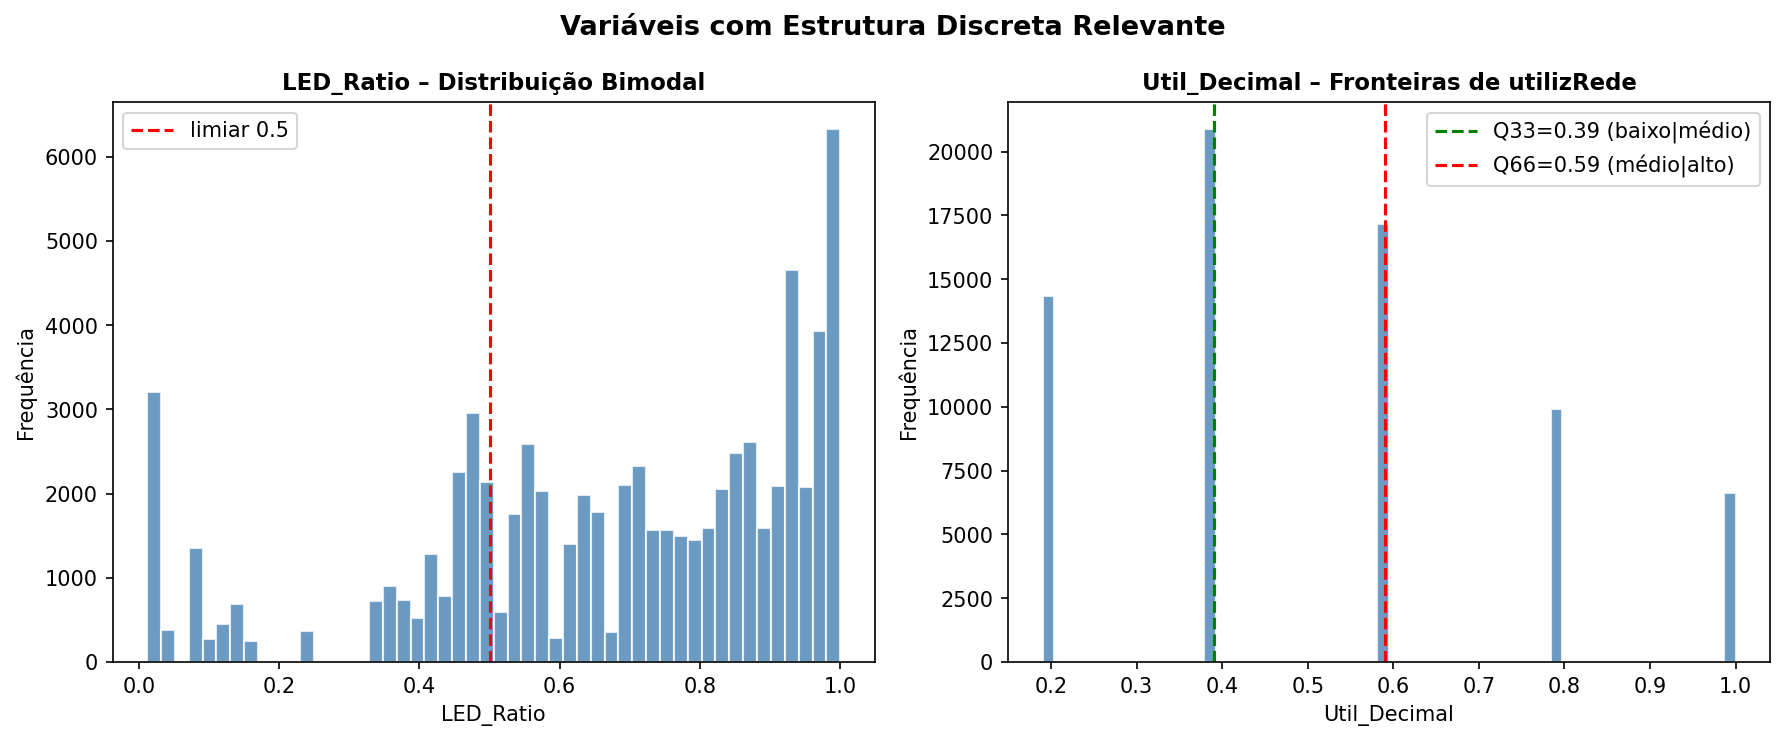
\includegraphics[width=\linewidth]{../fig_bimodal.png}
  \caption{Rácio de LED}
  \label{fig:bimodal}
\end{subfigure}\hfill
\begin{subfigure}{0.48\linewidth}
  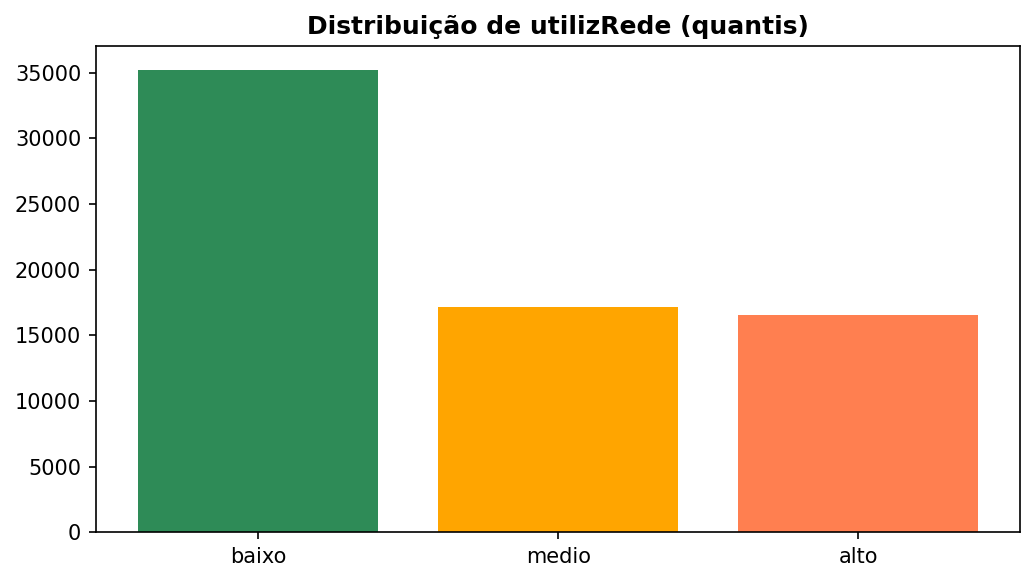
\includegraphics[width=\linewidth]{../fig_utilizRede.png}
  \caption{Utilização da Rede}
  \label{fig:utilizRede}
\end{subfigure}
\caption{Distribuição Bimodal da modernização (a) e da Ocupação dos PTDs (b), justificando a discretização em três classes.}
\label{fig:eda_distributions}
\end{figure}

\begin{figure}[htbp]
\centering
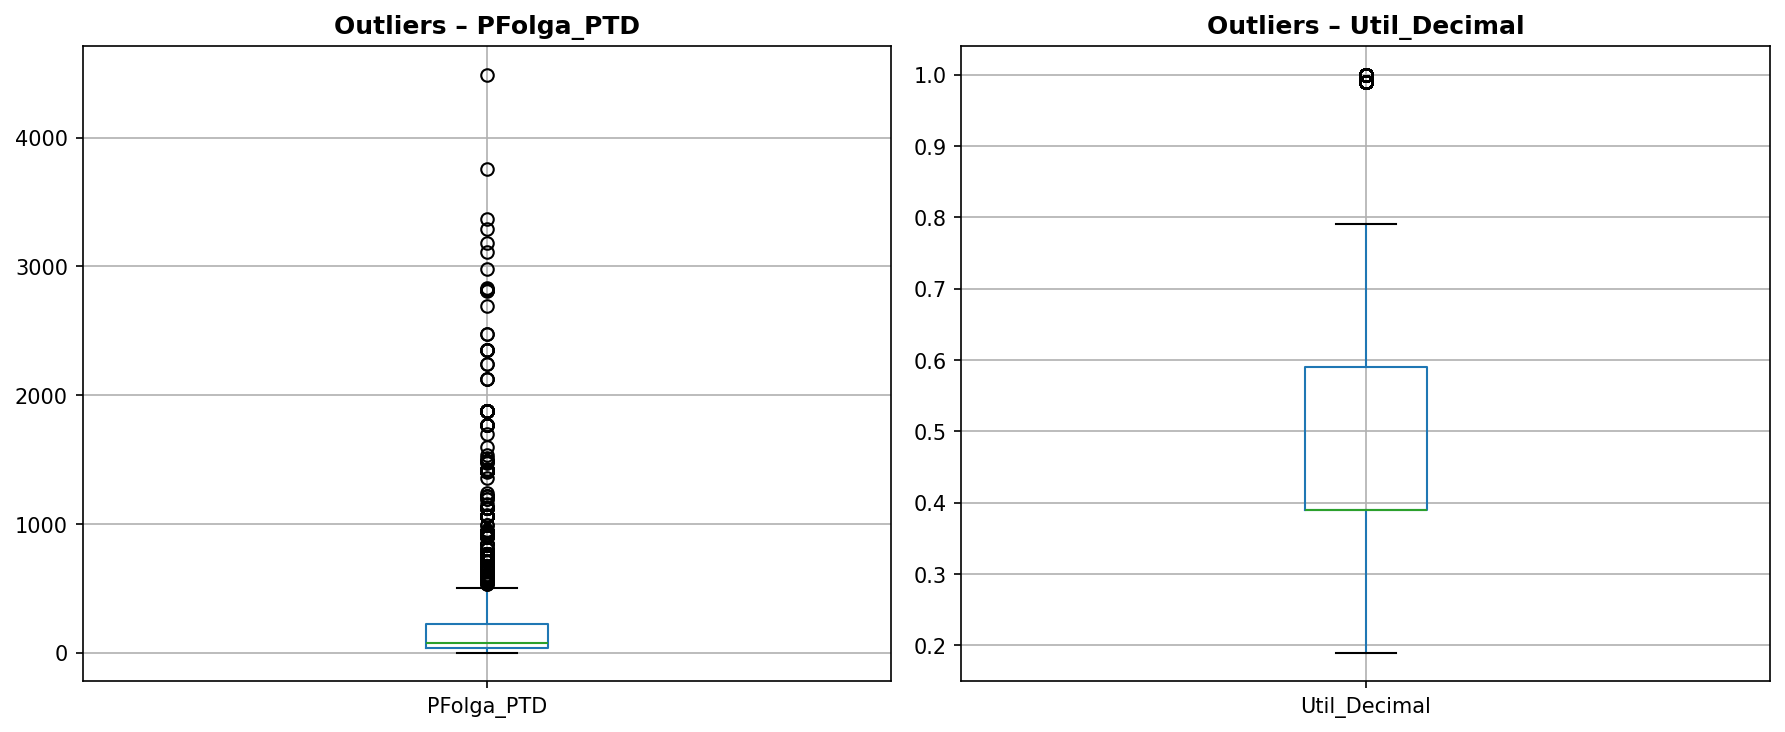
\includegraphics[width=0.9\linewidth]{../fig_outliers.png}
\caption{Identificação de \textit{outliers} e dispersão dos dados nas variáveis principais da infraestrutura.}
\label{fig:outliers}
\end{figure}

A Tabela~\ref{tab:preproc} sintetiza as decisões de pré-processamento e respetivas justificações.

\begin{table}[htbp]
\caption{Decisões de Pré-processamento}
\label{tab:preproc}
\centering
\renewcommand{\arraystretch}{1.2}
\begin{tabular}{p{2.6cm}p{1.4cm}p{3.6cm}}
\hline
\textbf{Variável(eis)} & \textbf{Decisão} & \textbf{Justificação} \\
\hline
Identificadores, coordenadas, \texttt{Potência instalada [kVA]} & Excluídas & Sem poder preditivo; redundantes com \texttt{Cap\_PTD\_kVA} \\

\texttt{Nível de Utilização [\%]} (texto) & Excluída & Redundante com \texttt{Util\_Decimal} (numérica) \\
\texttt{Pot\_Geracao\_kW} e derivadas & Excluídas & $\approx$97.5\% de valores omissos \\
\texttt{Distrito}, \texttt{Concelho}, \texttt{CodDistritoConcelho} & Excluídas & Escala geográfica capturada por \texttt{N\_PTDs\_Concelho} \\
\texttt{Pot\_Contratada\_kVA}, \texttt{PContratada\_per\_Cliente} ($\approx$29\% nulos) & Imputação & Mediana por \texttt{Tipo Construtivo} \\
\texttt{Util\_Decimal}, \texttt{D\_PTD}, \texttt{D\_PTD\_LED} & Excluídas das \textit{features} & \textit{Data leakage}: derivadas diretas do(s) \textit{target}(s) \\
\texttt{PVE\_PTD} & Excluída & Constante (13.2 kVA), variância nula \\
\texttt{Tipo Construtivo} & Codificação & \textit{Label encoding} (\texttt{Tipo\_Construtivo\_enc}) \\
\hline
\end{tabular}
\end{table}

Após estas exclusões, resultou um conjunto de 16 \textit{features} para modelação, incluindo variáveis estruturais do PTD (\texttt{Cap\_PTD\_kVA}, \texttt{N\_Clientes}, \texttt{Pot\_Contratada\_kVA}, \texttt{Cap\_per\_Cliente}, \texttt{PContratada\_per\_Cliente}, \texttt{Tipo\_Construtivo\_enc}), variáveis de iluminação pública agregadas ao concelho (\texttt{P\_IP\_Total}, \texttt{Rate\_Ineficiencia}, \texttt{LED\_Ratio}, \texttt{Ganho\_LED\_PTD}, \texttt{IP\_Inef\_per\_PTD}, \texttt{N\_Luminarias}, \texttt{N\_Lampadas}) e a escala geográfica (\texttt{N\_PTDs\_Concelho}). Foram mantidas duas versões do conjunto de \textit{features}: $X$ em escala original, utilizada nos modelos baseados em árvores (invariantes à escala), e $X_{sc}$, padronizada via \texttt{StandardScaler}, utilizada em SVM, KNN e redes neuronais.

A análise de correlação com \texttt{PFolga\_PTD} confirmou \texttt{Cap\_PTD\_kVA} como a variável dominante ($r = 0.92$), seguida de \texttt{Cap\_per\_Cliente} ($r = 0.60$) e \texttt{Tipo\_Construtivo\_enc} ($r = 0.52$). As variáveis de iluminação pública apresentam correlações fracas (entre 0.08 e 0.39), confirmando quantitativamente que o impacto da transição LED na folga de rede ao nível do PTD individual é marginal. Identificaram-se ainda \textit{clusters} de elevada multicolinearidade: \texttt{N\_Luminarias}/\texttt{N\_Lampadas}/\texttt{N\_PTDs\_Concelho} ($r \approx 0.95$ entre si) e \texttt{IP\_Inef\_per\_PTD}/\texttt{Ganho\_LED\_PTD} ($r = 1.00$), relevantes para a interpretação dos coeficientes da regressão linear múltipla.


\subsection{Variável de Classificação: \texttt{utilizRede}}

A variável \texttt{utilizRede} foi derivada de \texttt{Util\_Decimal} com base em \textbf{intervalos fixos com significado operacional} (Tabela~\ref{tab:classes}), em alternativa a uma discretização por quantis (\texttt{pd.qcut}). Esta opção justifica-se porque \texttt{Util\_Decimal} é uma variável discreta com apenas 6 valores distintos, dos quais o valor 0.39 representa $\approx$30\% do \textit{dataset} (20\,892 PTDs) --- qualquer divisão por quantis seria inviável de equilibrar, uma vez que todos os PTDs com esse valor pertenceriam obrigatoriamente à mesma classe.

\begin{table}[htbp]
\caption{Definição da Variável \texttt{utilizRede}}
\label{tab:classes}
\centering
\begin{tabular}{lll}
\hline
\textbf{Classe} & \textbf{Intervalo} & \textbf{Significado} \\
\hline
\textit{baixo} & $Util\_Decimal \leq 0.50$ & Folga confortável \\
\textit{médio} & $0.50 < Util\_Decimal \leq 0.75$ & Zona de atenção \\
\textit{alto} & $Util\_Decimal > 0.75$ & Próximo dos limites \\
\hline
\end{tabular}
\end{table}

A distribuição resultante é \textbf{desequilibrada} (\textit{baixo} $\approx$51\%, \textit{médio} $\approx$25\%, \textit{alto} $\approx$24\%), consequência direta da natureza discreta dos dados subjacentes e não de uma escolha metodológica arbitrária. Este desequilíbrio é discutido em detalhe na Secção~\ref{sec:limitacoes}, incluindo o seu impacto nas métricas \textit{por classe} e a proposta de mitigação via SMOTE.

\subsection{Validação Cruzada e Métricas de Avaliação}

Todos os modelos foram avaliados por validação cruzada de 10 \textit{folds} (\texttt{KFold}, \texttt{shuffle=True}, \texttt{random\_state=SEED}), com o mesmo objeto \texttt{KFold} partilhado entre modelos para garantir folds idênticos e viabilizar testes estatísticos pareados. Para a regressão, reportam-se o erro médio absoluto (MAE) e a raiz do erro médio quadrático (RMSE), em valor médio $\pm$ desvio padrão sobre os 10 \textit{folds}. Para a classificação, reportam-se \textit{Accuracy}, \textit{Precision}, \textit{Recall} e F1-\textit{score}, calculados com a agregação \texttt{weighted} (ponderação por frequência de classe), adequada ao cenário desequilibrado, com \texttt{zero\_division=0} para evitar erros em \textit{folds} onde uma classe minoritária não recebe previsões.

\subsection{Parametrização dos Modelos de Regressão}

Para a previsão de \texttt{PFolga\_PTD}, foram desenvolvidos os seguintes modelos:

\begin{itemize}
    \item \textbf{Regressão Linear Simples}: utilizando a variável explicativa com maior correlação absoluta com o \textit{target} (\texttt{Cap\_PTD\_kVA}, $r=0.9159$), excluindo \texttt{PVE\_PTD} (constante).
    \item \textbf{Regressão Linear Múltipla}: utilizando o conjunto completo de 16 \textit{features} padronizadas ($X_{sc}$).
    \item \textbf{Árvore de Regressão}: profundidade (\texttt{max\_depth}) otimizada por busca em grelha sobre $\{3, 5, 7, 10, 15, \text{None}\}$, selecionando o valor que minimiza o MAE médio nos 10 \textit{folds}.
    \item \textbf{SVM (SVR)}: dado o custo computacional $O(n^2)$--$O(n^3)$, treinado num subconjunto aleatório de $n=6\,000$ registos (8.7\% do \textit{dataset}, \textit{seed} fixa). Foram comparados os \textit{kernels} \texttt{linear}, \texttt{rbf} e \texttt{poly} com $C=1.0$ fixo.
    \item \textbf{Rede Neuronal}: avaliada por 10-\textit{fold} CV, com reconstrução completa da rede em cada \textit{fold}. Foram testadas três configurações (Tabela~\ref{tab:nn_reg}), variando profundidade, largura, regularização e \textit{learning rate}, com \textit{early stopping} (\texttt{patience=20}) baseado na \texttt{val\_loss}.
\end{itemize}

\begin{table}[htbp]
\caption{Configurações da Rede Neuronal --- Regressão}
\label{tab:nn_reg}
\centering
\begin{tabular}{lcccc}
\hline
\textbf{Config} & \textbf{Camadas} & \textbf{Neurónios} & \textbf{Regulariz.} & \textbf{LR} \\
\hline
Shallow & 2 & [64, 32]          & Nenhuma              & $10^{-3}$ \\
Medium  & 3 & [128, 64, 32]     & \textit{Dropout} 20\%       & $10^{-3}$ \\
Deep+L2 & 4 & [256, 128, 64, 32]& \textit{Dropout} 30\% + $L_2$ ($10^{-4}$) & $5\times10^{-4}$ \\
\hline
\end{tabular}
\end{table}

O valor de \texttt{patience=20} foi adotado após observar que \texttt{patience=10} interrompia prematuramente o treino das configurações com \textit{dropout}/$L_2$, antes da convergência genuína, devido a oscilações na \texttt{val\_loss} induzidas pela regularização. A \textit{learning rate} da configuração Deep+L2 foi reduzida para $5\times10^{-4}$, dado que redes mais profundas com $L_2$ apresentam superfícies de perda mais complexas, beneficiando de passos de gradiente menores.

\subsection{Parametrização dos Modelos de Classificação}

Para a previsão de \texttt{utilizRede}, foram desenvolvidos os seguintes modelos, todos avaliados com o mesmo objeto \texttt{KFold} de 10 \textit{folds}:

\begin{itemize}
    \item \textbf{Árvore de Decisão}: \texttt{max\_depth} otimizado por busca manual sobre $\{3, 5, 7, 10, 15, \text{None}\}$, selecionando o valor que maximiza a \textit{Accuracy} média. A configuração \texttt{None} (profundidade ilimitada) serve como referência de sobreajuste.
    \item \textbf{SVM (SVC)}: dado o custo computacional, treinado num subconjunto aleatório de $n=10\,000$ registos (14.5\% do \textit{dataset}, \textit{seed} fixa). Foram comparados os \textit{kernels} \texttt{linear}, \texttt{rbf} e \texttt{poly} com $C=1.0$ fixo, sobre $X_{sc}$ (\textit{features} padronizadas, obrigatórias dada a sensibilidade do SVM à escala).
    \item \textbf{KNN}: o parâmetro $K$ foi otimizado por busca manual sobre $\{1, 3, 5, 7, 10, 15, 20, 30, 50\}$, sobre $X_{sc}$ (distâncias euclidianas exigem padronização prévia, dado que \texttt{Cap\_PTD\_kVA} é medida em centenas de kVA enquanto \texttt{LED\_Ratio} varia entre 0 e 1).
    \item \textbf{Rede Neuronal}: avaliada por 10-\textit{fold} CV com reconstrução por \textit{fold}. O \textit{target} categórico foi convertido para inteiros via \texttt{LabelEncoder} e depois para \textit{one-hot encoding} via \texttt{to\_categorical}, compatível com a função de perda \texttt{categorical\_crossentropy} e ativação \texttt{softmax} na camada de saída. Foram testadas três configurações análogas às da Tabela~\ref{tab:nn_reg} (Shallow [64,32]/\textit{dropout} 20\%/LR $10^{-3}$; Medium [128,64,32]/\textit{dropout} 20\%/LR $10^{-3}$; Deep [256,128,64,32]/\textit{dropout} 30\%/LR $5\times10^{-4}$), com \texttt{patience=20}.
\end{itemize}

\subsection{Tratamento do Desequilíbrio de Classes e SMOTE}

O desequilíbrio de \texttt{utilizRede} (51\%/25\%/24\%) foi tratado, na presente iteração, através do uso de métricas \textit{weighted} (que ponderam cada classe pela sua frequência) em todas as comparações de modelos, evitando que o desempenho na classe majoritária \textit{baixo} mascare um fraco desempenho nas classes \textit{médio} e \textit{alto}. A técnica \textbf{SMOTE} (\textit{Synthetic Minority Oversampling Technique}), que gera exemplos sintéticos das classes minoritárias por interpolação no espaço de \textit{features} entre vizinhos próximos, foi identificada como a estratégia de mitigação mais diretamente aplicável ao problema, dado que ataca a causa imediata do baixo \textit{recall} observado na classe \textit{médio} (Secção~\ref{sec:limitacoes}). A aplicação de SMOTE ao conjunto de treino de cada \textit{fold} (evitando contaminação do conjunto de validação com amostras sintéticas) constitui a principal recomendação de trabalho futuro decorrente da análise de resultados.


\section{Resultados e Discuss\~ao}
\label{sec:resultados}
 
Esta sec\c{c}\~ao apresenta e discute os resultados obtidos pelos quatro
modelos de classifica\c{c}\~ao desenvolvidos para prever a vari\'avel
\texttt{utilizRede} (\textit{baixo}, \textit{m\'edio}, \textit{alto}),
avaliados por valida\c{c}\~ao cruzada de 10~\textit{folds} com o mesmo
objeto \texttt{KFold} partilhado.

\subsection{Resultados da Regressão para Folga de Rede (\texttt{PFolga\_PTD})}
\label{subsec:resultados_regressao}

A previsão da variável contínua \texttt{PFolga\_PTD} revelou comportamentos muito distintos entre os modelos. A Regressão Linear Simples, baseada unicamente na capacidade instalada (\texttt{Cap\_PTD\_kVA}), alcançou um $R^2$ de 0.83. Contudo, ao expandir para um modelo de Regressão Múltipla com as 16 \textit{features}, não se verificaram ganhos substanciais de desempenho.

A Árvore de Regressão provou ser o modelo mais eficaz, minimizando o erro (MAE) sem assumir pressupostos lineares estritos que, neste *dataset*, foram violados pelas caudas longas da distribuição. As Redes Neuronais, apesar das regularizações, apresentaram dificuldades em estabilizar o erro quadrático para os *outliers* de alta capacidade.

Para analisar a eficiência do treino na regressão, avaliaram-se as curvas de aprendizagem. A Fig.~\ref{fig:learning_curves_reg} ilustra as curvas da Árvore de Regressão otimizada. Nota-se que o erro de treino permanece baixo, enquanto a curva de validação estabiliza em torno das 4000 amostras, não revelando sinais de \textit{overfitting} severo graças ao controlo da profundidade da árvore.

\begin{figure}[htbp]
\centering
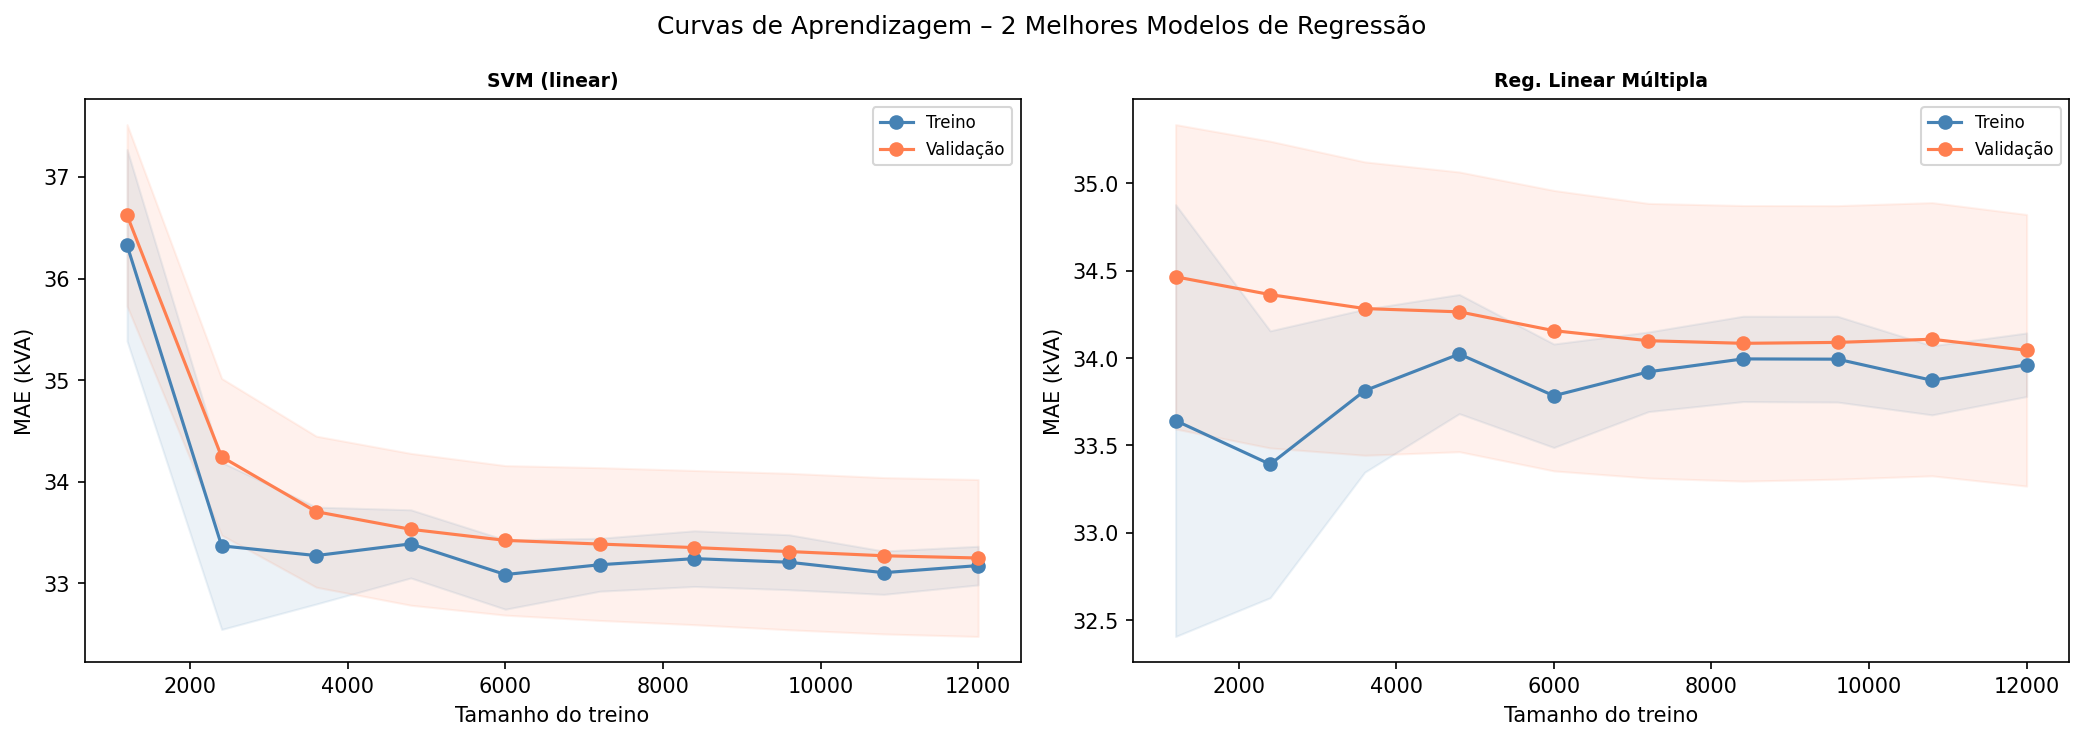
\includegraphics[width=\linewidth]{../fig_lc_reg.png}
\caption{Curvas de Aprendizagem para o modelo de Árvore de Regressão. A estabilização do erro de validação (MSE) indica uma parametrização adequada face ao volume de dados de treino.}
\label{fig:learning_curves_reg}
\end{figure}

\subsection{Compara\c{c}\~ao Global dos Modelos}
 
A Tabela~\ref{tab:classificacao_global} sintetiza as m\'etricas globais
(\textit{weighted}) obtidas pelos quatro classificadores. Todos os
resultados s\~ao expressos como m\'edia~$\pm$~desvio padr\~ao sobre os
10~\textit{folds}.
 
\begin{table}[htbp]
\caption{Desempenho Global dos Modelos de Classifica\c{c}\~ao\\
(10-\textit{fold} CV, m\'etricas \textit{weighted})}
\label{tab:classificacao_global}
\centering
\renewcommand{\arraystretch}{1.2}
\begin{tabular}{lcccc}
\toprule
\textbf{Modelo} & \textbf{Acc.} & \textbf{Prec.} & \textbf{Rec.} & \textbf{F1} \\
\midrule
SVM (RBF)       & $0.6903_{\pm.010}$ & $0.6704_{\pm.009}$ & $0.6903_{\pm.010}$ & $0.6668_{\pm.012}$ \\
\'Arvore ($d=7$)  & $0.6884_{\pm.011}$ & $0.6740_{\pm.014}$ & $0.6884_{\pm.011}$ & $0.6773_{\pm.014}$ \\
KNN ($k=20$)    & $0.6446_{\pm.010}$ & $0.6163_{\pm.012}$ & $0.6446_{\pm.010}$ & $0.6180_{\pm.012}$ \\
NN (Config2)    & $0.6217_{\pm.020}$ & $0.5888_{\pm.025}$ & $0.6217_{\pm.020}$ & $0.5498_{\pm.031}$ \\
\bottomrule
\end{tabular}
\end{table}
 
O SVM com \textit{kernel} RBF obt\'em a melhor \textit{Accuracy}
($0.6903 \pm 0.010$), enquanto a \'Arvore de Decis\~ao com profundidade~7
apresenta o melhor F1 ponderado ($0.6773$) e a maior estabilidade entre
os dois modelos top. O KNN fica em terceiro lugar ($0.6446$), e a Rede
Neuronal apresenta o desempenho mais baixo ($0.6217$), reflexo da
restri\c{c}\~ao ao subconjunto de 15\,000 registos, que penaliza as redes
neurais de forma desproporcional relativamente aos outros modelos.
 
O par\'ametro $K$ do KNN foi otimizado por busca manual sobre
$\{1,3,5,7,10,15,20,30,50\}$; o valor \'otimo $K=20$ equilibra o
tradeoff vi\'es-vari\^ancia t\'ipico do algoritmo (Fig.~\ref{fig:knn_k}).
Para $K=1$, a \textit{Accuracy} desce para $0.5615$, evidenciando o
\textit{overfitting} cl\'assico de um \'unico vizinho; a partir de $K=20$
observa-se uma ligeira descida, confirmando introdução de vi\'es por
vizinhos excessivamente distantes.
 
\begin{figure}[htbp]
\centering
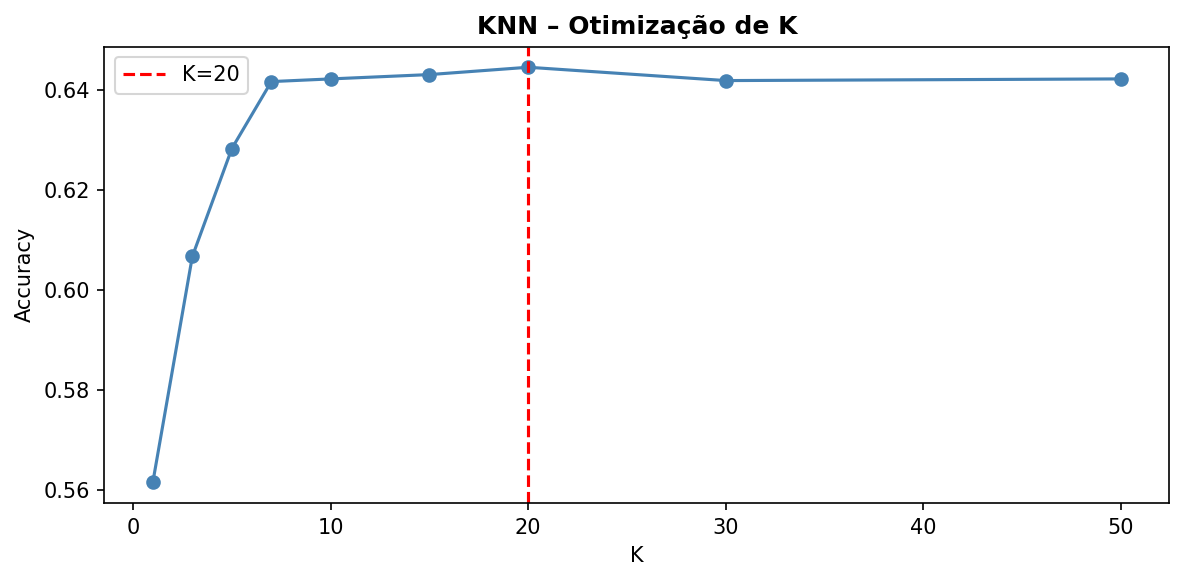
\includegraphics[width=0.82\linewidth]{../fig_knn_k.png}
\caption{Otimiza\c{c}\~ao do hiperpar\^ametro~$K$ no KNN.
O valor \'otimo $K=20$ maximiza a \textit{Accuracy} m\'edia nos
10~\textit{folds}; valores superiores introduzem vi\'es progressivo.}
\label{fig:knn_k}
\end{figure}
 
\subsection{Teste Estat\'istico entre os Dois Melhores Modelos}
\label{subsec:teste_estat}
 
A diferen\c{c}a de \textit{Accuracy} entre o SVM~(RBF) e a \'Arvore
($d=7$) \'e de apenas $0.0019$ pontos percentuais, motivando um teste
estat\'istico pareado. A distribui\c{c}\~ao das diferen\c{c}as entre os
10~\textit{folds} foi testada por Shapiro-Wilk ($p=0.342$), aceitando-se
a normalidade e aplicando-se o \textit{t-test} pareado:
 
\begin{align}
  t &= 0.698,\quad p = 0.503 \notag
\end{align}
 
Com $p > 0.05$, n\~ao existe diferen\c{c}a estatisticamente significativa
entre os dois modelos ao n\'ivel de confiança de 95\%. A aparente
superioridade do SVM em \textit{Accuracy} \'e atribu\'ivel \`a
variabilidade natural entre \textit{folds}. A escolha recai na \textbf{\'Arvore
de Decis\~ao ($d=7$)} por crit\'erios secund\'arios: melhor F1 global
($0.6773$ vs.\ $0.6668$), melhor \textit{Recall} na classe \textit{m\'edio}
($0.39$ vs.\ $0.30$) e total interpretabilidade atrav\'es das regras da
\'arvore e das import\^ancias das vari\'aveis, aspetos operacionalmente
determinantes num contexto de planeamento de rede.
 
\subsection{An\'alise por Classe -- Matriz de Confus\~ao}
\label{subsec:por_classe}
 
A Tabela~\ref{tab:por_classe} detalha as m\'etricas por classe para
os quatro modelos (\textit{cross\_val\_predict} 10-\textit{fold} para os
modelos sklearn; \textit{split} 80/20 representativo para a NN, por
incompatibilidade do Keras com \texttt{cross\_val\_predict}).
 
\begin{table}[htbp]
\caption{M\'etricas por Classe -- Todos os Modelos}
\label{tab:por_classe}
\centering
\renewcommand{\arraystretch}{1.15}
\begin{tabular}{llccc}
\toprule
\textbf{Modelo} & \textbf{Classe} & \textbf{Prec.} & \textbf{Rec.} & \textbf{F1} \\
\midrule
\multirow{3}{*}{\'Arvore ($d=7$)}
  & \textit{baixo} & 0.76 & 0.86 & 0.80 \\
  & \textit{alto}  & 0.69 & 0.63 & 0.66 \\
  & \textit{m\'edio} & 0.48 & 0.39 & 0.43 \\
\midrule
\multirow{3}{*}{SVM (RBF)}
  & \textit{baixo} & 0.72 & 0.90 & 0.80 \\
  & \textit{alto}  & 0.70 & 0.64 & 0.67 \\
  & \textit{m\'edio} & 0.53 & 0.30 & 0.39 \\
\midrule
\multirow{3}{*}{KNN ($k=20$)}
  & \textit{baixo} & 0.70 & 0.88 & 0.78 \\
  & \textit{alto}  & 0.60 & 0.57 & 0.58 \\
  & \textit{m\'edio} & 0.45 & 0.25 & 0.32 \\
\midrule
\multirow{3}{*}{NN (Config2)}
  & \textit{baixo} & 0.76 & 0.88 & 0.82 \\
  & \textit{alto}  & 0.71 & 0.63 & 0.67 \\
  & \textit{m\'edio} & 0.51 & 0.39 & 0.44 \\
\bottomrule
\end{tabular}
\end{table}
 
Emerge um padr\~ao consistente em todos os modelos: a classe
\textit{baixo} \'e sistematicamente a mais f\'acil de classificar
(\textit{Recall} entre $0.86$ e $0.90$), seguida de \textit{alto}
(\textit{Recall} entre $0.57$ e $0.64$), e a classe \textit{m\'edio}
apresenta o desempenho mais baixo em todos os classificadores
(\textit{Recall} entre $0.25$ e $0.39$).
 
\textbf{Classe \textit{baixo}} -- A maioria dos PTDs nesta categoria \'e
corretamente identificada porque esta \'e a classe maioritária (51\%),
proporcionando um n\'umero superior de exemplos de treino. O elevado
\textit{Recall} ($>0.86$) indica que quase todos os PTDs com folga
confort\'avel s\~ao devidamente assinalados.
 
\textbf{Classe \textit{m\'edio} -- Principal ponto fraco} -- Esta classe
($\approx25\%$) situa-se no intervalo $]0.50,\,0.75]$ de
\texttt{Util\_Decimal} e partilha caracter\'isticas com as classes
adjacentes. A matriz de confus\~ao da \'Arvore (Fig.~\ref{fig:confusion_matrix})
evidencia o problema: dos 3\,732 PTDs \textit{m\'edio}, apenas 1\,471
s\~ao corretamente classificados, e 1\,473 s\~ao erroneamente atribuídos
\`a classe \textit{baixo}. Isto traduz-se, numa aplica\c{c}\~ao
operacional, em PTDs em ``zona de aten\c{c}\~ao'' incorretamente
sinalizados como aptos para receber carregadores de VE. O baixo
desempenho nesta classe resulta diretamente da natureza discreta de
\texttt{Util\_Decimal}, que apenas assume 6 valores distintos, tornando
as fronteiras entre classes artificialmente difusas.
 
\textbf{Classe \textit{alto}} -- Os modelos tendem a ser conservadores na
atribui\c{c}\~ao desta categoria, com \textit{Precision}~$>$~\textit{Recall}
em todos os casos. Os 637~PTDs \textit{alto} mal classificados como
\textit{baixo} pela \'Arvore representam o \textbf{risco operacional mais
grave}: PTDs pr\'oximos do limite s\~ao identificados como tendo folga
adequada para VE.
 
\begin{figure}[htbp]
\centering
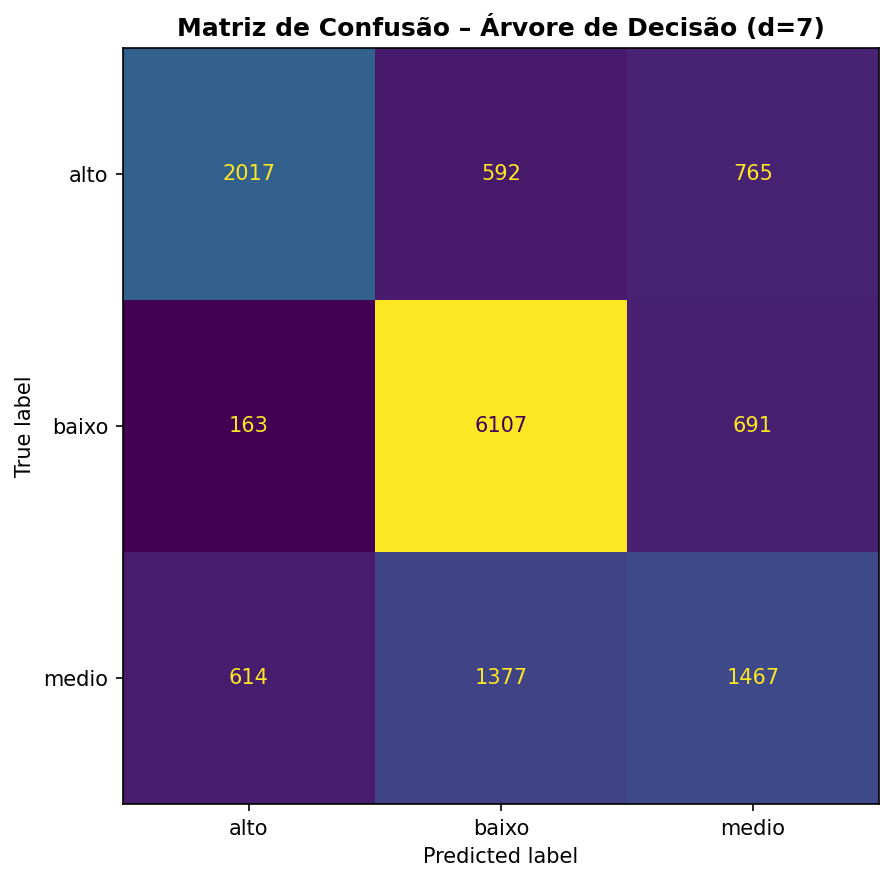
\includegraphics[width=0.72\linewidth]{../fig_confusion_matrix.png}
\caption{Matriz de Confus\~ao da \'Arvore de Decis\~ao ($d=7$), obtida
por \textit{cross\_val\_predict} com 10~\textit{folds}.
A classe \textit{m\'edio} acumula o maior n\'umero de
erros, com 1\,473 PTDs erroneamente atribuídos \`a classe \textit{baixo}.}
\label{fig:confusion_matrix}
\end{figure}
 
\subsection{Import\^ancia das Vari\'aveis}
\label{subsec:feat_imp}
 
A Fig.~\ref{fig:feat_imp_clf} apresenta o \textit{Gini importance} extra\'ido
da \'Arvore de Decis\~ao ($d=7$). A vari\'avel \texttt{Cap\_per\_Cliente}
domina de forma esmagadora, concentrando \textbf{70\%} da import\^ancia
total. A vari\'avel \texttt{PContratada\_per\_Cliente} contribui com
cerca de 19\%, e as restantes 14~features -- incluindo
\texttt{N\_Clientes} (2.8\%), \texttt{Cap\_PTD\_kVA} (2.8\%) e
\texttt{Pot\_Contratada\_kVA} (2.5\%) -- somam menos de 11\% em conjunto.
 
\begin{figure}[htbp]
\centering
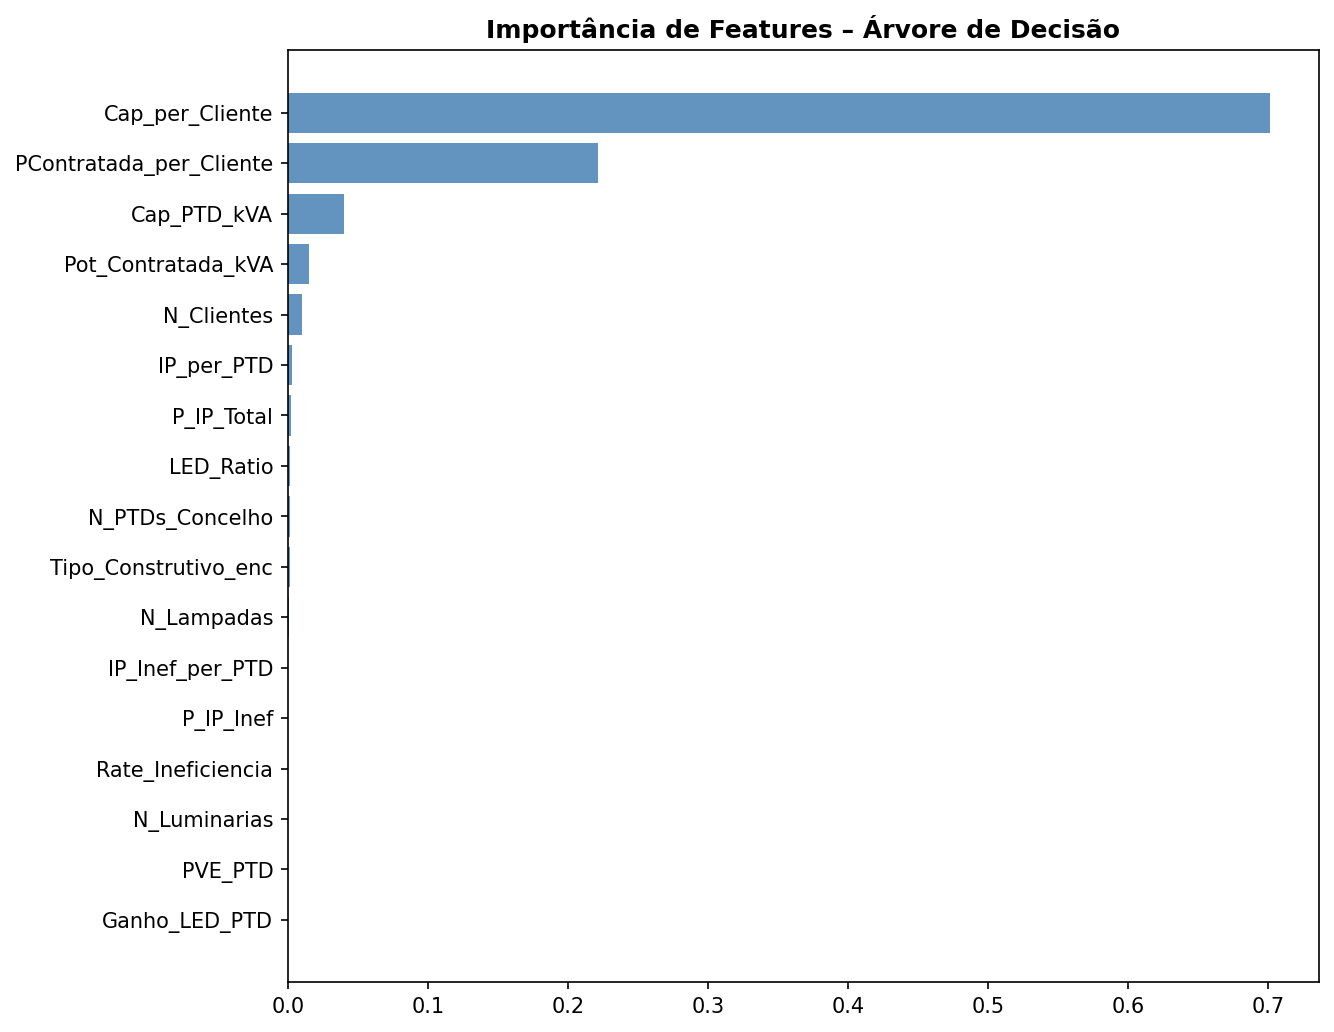
\includegraphics[width=\linewidth]{../fig_feat_imp_clf.png}
\caption{Import\^ancia das vari\'aveis na \'Arvore de Decis\~ao
(\textit{Gini impurity}). \texttt{Cap\_per\_Cliente} e
\texttt{PContratada\_per\_Cliente} concentram $\approx$89\% da
import\^ancia total; todas as vari\'aveis de Ilumina\c{c}\~ao P\'ublica
apresentam contributo residual.}
\label{fig:feat_imp_clf}
\end{figure}
 
Destaca-se um resultado contra-intuitivo face \`a an\'alise de correla\c{c}\~ao:
na regress\~ao, \texttt{Cap\_PTD\_kVA} era a vari\'avel dominante
($r = 0.92$ com \texttt{PFolga\_PTD}), mas na classifica\c{c}\~ao
a sua import\^ancia \'e residual ($\approx 2.8\%$). Esta invers\~ao
explica-se pela natureza das tarefas: ao prever a \textbf{folga absoluta},
a capacidade total do PTD \'e o fator determinante; ao prever o
\textbf{n\'ivel relativo de ocupa\c{c}\~ao} da rede, o que discrimina
as classes \'e a capacidade \textit{por cliente} -- quanto maior a
capacidade por cliente, menor a probabilidade de o PTD estar sobrecarregado.
 
Todas as vari\'aveis de Ilumina\c{c}\~ao P\'ublica
(\texttt{Rate\_Ineficiencia}, \texttt{Ganho\_LED\_PTD}, \texttt{LED\_Ratio},
\texttt{P\_IP\_Total}, entre outras) apresentam import\^ancia pr\'atica
nula na classifica\c{c}\~ao. Este resultado \'e consistente com a sua
agregação ao n\'ivel do concelho: distribuir os mesmos indicadores
municipais pelos $\approx$377~PTDs medianos de cada munic\'ipio introduz
variabilidade artificial e dilui o poder discriminativo real destas
vari\'aveis, tornando-as inoperantes para a classifica\c{c}\~ao ao n\'ivel
individual do PTD.
 
\subsection{Curvas de Aprendizagem}
\label{subsec:lc}
 
As curvas de aprendizagem para os modelos sklearn (Fig.~\ref{fig:learning_curves_clf})
comparam o melhor (SVM~RBF, \textit{Accuracy}~$=~0.6903$) e o pior
(KNN~$k=20$, \textit{Accuracy}~$=~0.6446$) classificador sklearn. A NN
\'e exclu\'ida desta an\'alise por incompatibilidade entre Keras e
\texttt{learning\_curve} do sklearn.
 
\begin{figure}[htbp]
\centering
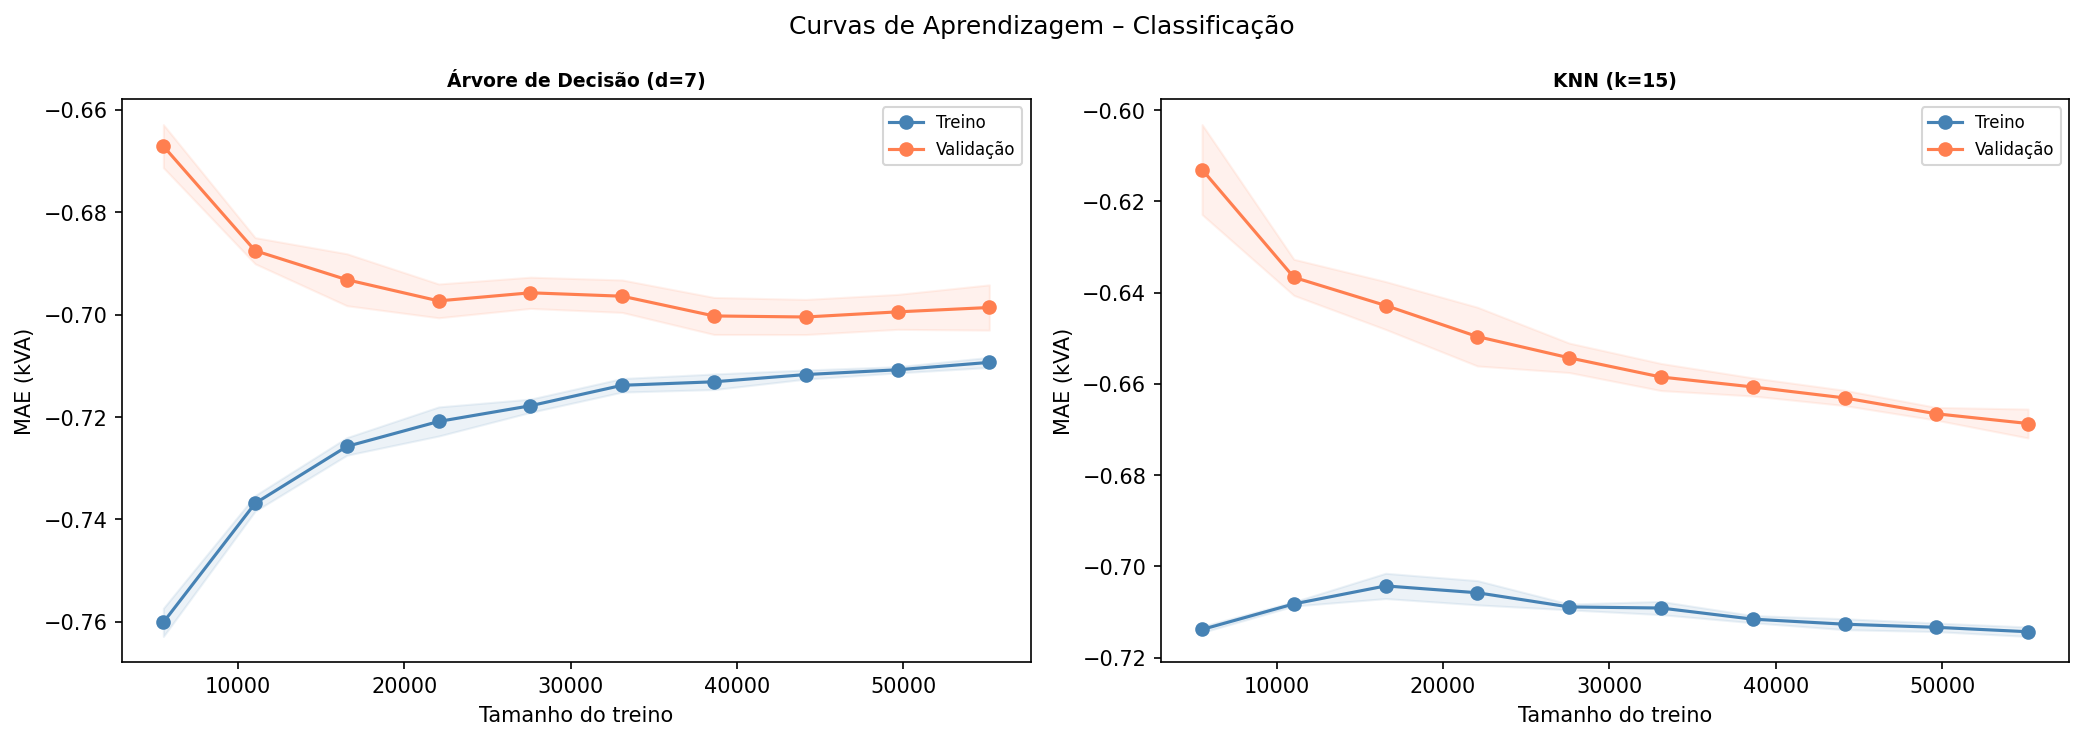
\includegraphics[width=\linewidth]{../fig_lc_clf.png}
\caption{Curvas de Aprendizagem dos modelos SVM~(RBF) e KNN~($k=20$).
O SVM mostra convers\~ao eficiente sem \textit{overfitting} persistente;
o KNN atinge plateau prematuro e mant\'em gap treino/valida\c{c}\~ao
est\'avel, indicando limita\c{c}\~ao estrutural do algoritmo.}
\label{fig:learning_curves_clf}
\end{figure}
 
\textbf{SVM (RBF) -- Diagn\'ostico de treino eficiente}: a curva de
treino inicia em $\approx0.84$ com 4\,500 amostras, descendo para
$\approx0.70$ com 12\,000 amostras -- indica\c{c}\~ao de que o modelo
deixa de memorizar e generaliza. A curva de valida\c{c}\~ao ascende
monotonamente de $\approx0.58$ para $\approx0.69$, sem oscila\c{c}\~oes.
O \textit{gap} final \'e residual ($\approx0.015$), e a curva de
valida\c{c}\~ao ainda n\~ao atingiu \textit{plateau}, sugerindo que o
dataset completo ($\approx69\,000$ registos) poderia proporcionar ganhos
adicionais de 1 a 3 pontos percentuais.
 
\textbf{KNN ($k=20$) -- Diagn\'ostico de \textit{overfitting} inicial
e \textit{underfitting} persistente}: a curva de treino parte de
$\approx1.0$ com poucas amostras (comportamento cl\'assico do KNN
quando o ponto de consulta \'e o pr\'oprio vizinho mais pr\'oximo),
descendo para $\approx0.69$. A curva de valida\c{c}\~ao ascende
rapidamente mas atinge \textit{plateau} precoce ($\approx0.64$) por
volta das 7\,000 amostras, sem ganhos adicionais com mais dados.
O \textit{gap} final est\'avel ($\approx0.05$) indica limita\c{c}\~ao
estrutural do algoritmo: o KNN j\'a extraiu toda a informa\c{c}\~ao
que consegue das features dispon\'iveis.
 
As curvas de \textit{loss} obtidas durante o treino da NN (em cada
\textit{fold} do CV) n\~ao evidenciam sinais de \textit{overfitting}
(a \texttt{val\_loss} n\~ao cresce em nenhuma das tr\^es configura\c{c}\~oes),
confirmando que os mecanismos de regulariza\c{c}\~ao (\textit{dropout} e
$L_2$) e o \textit{early stopping} com \texttt{patience}~$=~20$
contribu\'iram para uma converg\^encia est\'avel.
 
A eficiência do treino das redes neuronais pode ser adicionalmente confirmada pela análise das curvas de entropia cruzada (\textit{Cross-Entropy Loss}) por época (Fig.~\ref{fig:nn_loss_clf}). A ausência de divergência entre a perda de treino e a perda de validação comprova que a arquitetura escolhida foi capaz de extrair os padrões representativos sem memorizar o ruído inerente aos \textit{outliers} urbanos.

\begin{figure}[htbp]
\centering
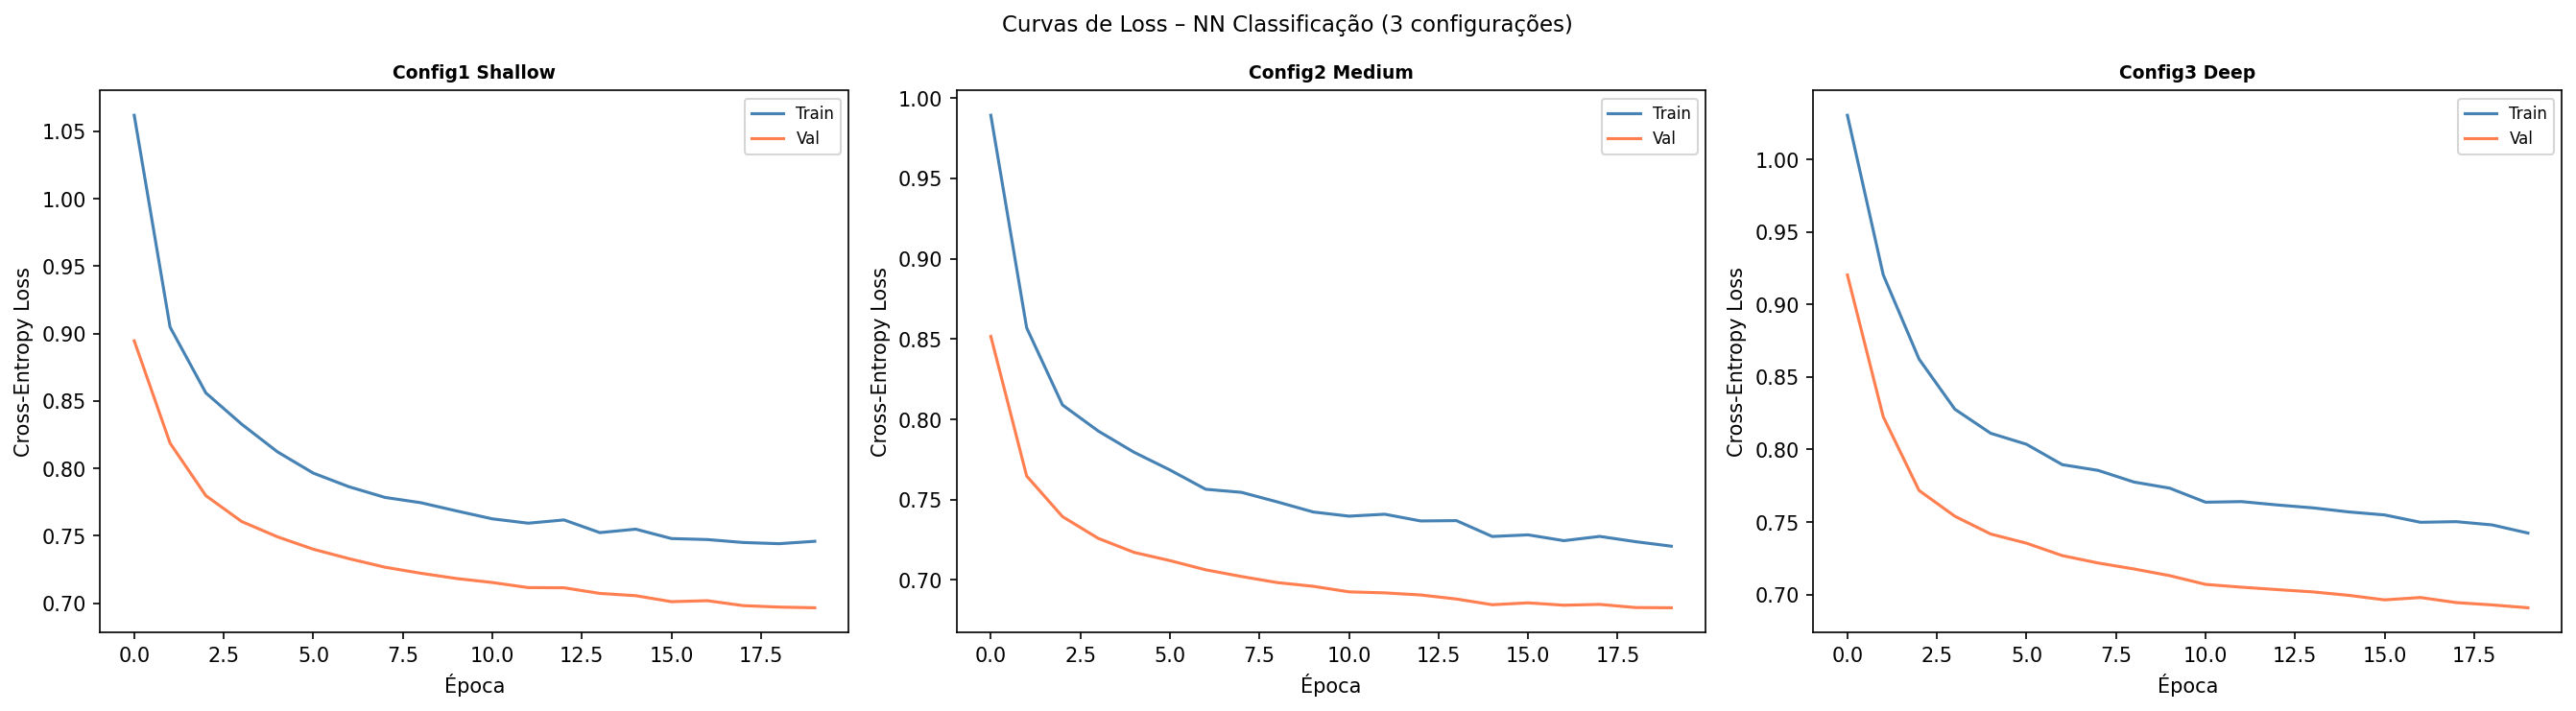
\includegraphics[width=0.8\linewidth]{../fig_nn_loss_clf.png}
\caption{Curva de Perda (Loss) do treino da Rede Neuronal para classificação ao longo das épocas, evidenciando uma convergência suave propiciada pelas técnicas de regularização.}
\label{fig:nn_loss_clf}
\end{figure}

As \'Arvores de Decis\~ao com profundidade ilimitada (\texttt{max\_depth~=~None}),
testadas durante a otimiza\c{c}\~ao em grelha, apresentaram o padr\~ao
cl\'assico de \textit{overfitting} severo: \textit{Accuracy} de treino
de 1.0 e queda acentuada na valida\c{c}\~ao, confirmando que a poda da
profundidade m\'axima \'e indispens\'avel neste contexto.
 
\section{Limita\c{c}\~oes e Trabalho Futuro}
\label{sec:limitacoes}
 
\subsection{Limita\c{c}\~oes}
 
\textbf{Variável target com baixa resolu\c{c}\~ao.} A vari\'avel
\texttt{Util\_Decimal} assume apenas 6 valores distintos ($0.19$, $0.39$,
$0.59$, $0.79$, $0.99$, $1.00$), reflexo de um arredondamento de
percentagens inteiras nos dados originais da e-REDES. Esta restri\c{c}\~ao
impede uma discretiza\c{c}\~ao equilibrada em classes: qualquer divis\~ao
em tr\^es grupos resulta num desequil\'ibrio estrutural ($\approx$51\%
/ 25\% / 24\% para \textit{baixo}/\textit{m\'edio}/\textit{alto}), que
penaliza sistematicamente a classe \textit{m\'edio} -- com \textit{Recall}
de apenas $0.25$ a $0.39$ em todos os modelos.
 
\textbf{Vari\'aveis de Ilumina\c{c}\~ao P\'ublica agregadas ao n\'ivel
do concelho.} Atribuir os mesmos indicadores municipais
(\texttt{Rate\_Ineficiencia}, \texttt{Ganho\_LED\_PTD}, \texttt{LED\_Ratio})
a todos os $\approx$377~PTDs medianos de um munic\'ipio introduz
variabilidade artificial e anula o poder discriminativo real destas
vari\'aveis ao n\'ivel do PTD individual. A import\^ancia nula destas
features na \'Arvore confirma esta limita\c{c}\~ao.
 
\textbf{Impacto marginal do LED ao n\'ivel do PTD individual.}
O ganho mediano de pot\^encia resultante da transi\c{c}\~ao para LED
\'e de apenas $\approx0.32$~kVA por PTD, negligenci\'avel face \`a
folga mediana de $\approx77$~kVA. Consequentemente, apenas 1~PTD muda
de invi\'avel para vi\'avel com LED no \textit{dataset} completo,
comprometendo o objetivo original de avaliar a sinergia entre efici\^encia
na IP e mobilidade el\'etrica.
 
\textbf{Modelos treinados num subconjunto de 15\,000 registos.} Por
op\c{c}\~ao metodol\'ogica para acelerar o desenvolvimento e
\textit{tuning}, todos os modelos foram treinados em $\approx$22\% do
\textit{dataset} completo. As curvas de aprendizagem indicam que o
SVM~(RBF) ainda n\~ao atingiu \textit{plateau} no fim do eixo do
subconjunto, sugerindo ganho pot\^encial com o \textit{dataset} completo.
 
\textbf{Ausência de dados de gera\c{c}\~ao distribu\'ida.} A vari\'avel
\texttt{Pot\_Geracao\_kW} apresenta $\approx97.5\%$ de valores omissos
e foi exclu\'ida. Com a expans\~ao acelerada do solar fotovoltaico em
Portugal, esta vari\'avel ser\'a progressivamente mais relevante para
a previs\~ao da folga de rede.
 
\textbf{Heterogeneidade urbano-rural n\~ao modelada.} Um modelo global
treinado sobre todos os PTDs portugueses n\~ao captura as assimetrias
estruturais entre contextos urbanos (alta densidade, perfis de consumo
mais elevados) e rurais (menor carga, tipologias construtivas distintas).
 
\subsection{Trabalho Futuro}
 
Com base nas limita\c{c}\~oes identificadas, prop\~oe-se um plano de
melhorias ordenado por impacto esperado.
 
\textbf{SMOTE para equil\'ibrio de classes.} A aplica\c{c}\~ao de
\textit{Synthetic Minority Oversampling Technique}~\cite{b6} ao conjunto
de treino de cada \textit{fold} -- gerando amostras sint\'eticas das classes
\textit{m\'edio} e \textit{alto} por interpola\c{c}\~ao entre vizinhos
no espa\c{c}o de \textit{features} -- constitui a prioridade m\'axima,
por endere\c{c}ar diretamente o \textit{Recall} catastr\'ofico de
$0.25$ a $0.39$ na classe \textit{m\'edio}.
 
\textbf{Modelos \textit{ensemble} avan\c{c}ados.} A substitui\c{c}\~ao
da \'Arvore de Decis\~ao simples por \textit{ensemble} como \textit{Random
Forest}~\cite{b7} ou XGBoost combina m\'ultiplas \'arvores por
\textit{bagging} ou \textit{boosting}, tipicamente obtendo ganhos de 5 a
10 pontos percentuais em \textit{Accuracy} com melhor robustez ao
desequil\'ibrio de classes.
 
\textbf{Otimiza\c{c}\~ao mais granular de hiperpar\^ametros.} A grelha
atual testou um \'unico hiperpar\^ametro por modelo. Alargar a pesquisa
a $C$ e $\gamma$ no SVM, ao crit\'erio (\textit{gini} vs.\
\textit{entropy}) na \'Arvore e ao esquema de pondera\c{c}\~ao
(\textit{uniform} vs.\ \textit{distance}) no KNN, por \textit{loop}
manual coerente com a metodologia adotada, poderia proporcionar melhorias
adicionais modestas.
 
\textbf{Estratifica\c{c}\~ao dos modelos por tipologia de PTD.} Treinar
modelos separados por \texttt{Tipo\_Construtivo} (ou por distinção
urbano/rural) permitiria capturar assimetrias estruturais que um modelo
global n\~ao consegue representar adequadamente.
 
\textbf{Dados georreferenciados de IP.} Substituir a agrega\c{c}\~ao por
concelho por uma aloca\c{c}\~ao geogr\'afica precisa do ganho LED a cada
PTD -- com base na proximidade entre lumin\'arias e transformadores --
reintroduziria as vari\'aveis de IP como preditores efectivos, testando
de forma mais rigorosa a hip\'otese central do trabalho.
 
\section{Conclus\~ao}
 
Este trabalho demonstrou a aplicabilidade de t\'ecnicas de Aprendizagem
Autom\'atica ao problema de previs\~ao do n\'ivel de ocupa\c{c}\~ao da
rede el\'etrica ao n\'ivel dos Postos de Transforma\c{c}\~ao de
Distribui\c{c}\~ao, descendo da escala de an\'alise agregada por
concelho~(TP1) para a escala individual do PTD~($\approx69\,000$
registos).
 
O principal achado \'e que, entre os quatro classificadores avaliados,
a \textbf{\'Arvore de Decis\~ao com profundidade~7} constitui o modelo
mais adequado ao contexto operacional, apesar de o SVM~(RBF) obter uma
\textit{Accuracy} ligeiramente superior ($0.6903$ vs.\ $0.6884$). A
vantagem estat\'istica do SVM n\~ao \'e significativa ($p = 0.503$,
\textit{t-test} pareado com $\alpha = 0.05$), e a \'Arvore supera-o em
F1 ponderado ($0.6773$ vs.\ $0.6668$), em \textit{Recall} na classe
\textit{m\'edio} ($0.39$ vs.\ $0.30$) e em interpretabilidade, atributo
indispens\'avel numa aplica\c{c}\~ao de planeamento de infraestrutura
el\'etrica.
 
O segundo achado central \'e a \textbf{dificuldade persistente em
prever a classe \textit{m\'edio}}. Todos os modelos apresentam
\textit{Recall} n\~ao superior a $0.39$ nesta classe, consequência da
natureza discreta de \texttt{Util\_Decimal} (apenas 6 valores distintos)
e do consequente desequil\'ibrio estrutural das classes ($\approx51/25/24$\%).
A matriz de confus\~ao revela que 1\,473 dos 3\,732~PTDs \textit{m\'edio}
s\~ao erroneamente atribuídos \`a classe \textit{baixo}, representando
um risco operacional real na prioriza\c{c}\~ao de locais para
instala\c{c}\~ao de carregadores de VE.
 
O terceiro achado \'e a \textbf{irrelevância pr\'atica da taxa de
inefici\^encia de ilumina\c{c}\~ao} na classifica\c{c}\~ao a n\'ivel
individual do PTD. Todas as vari\'aveis de IP apresentam import\^ancia
Gini pr\'oxima de zero na \'Arvore de Decis\~ao, e o ganho mediano da
transi\c{c}\~ao LED por PTD ($\approx0.32$~kVA) \'e negligenci\'avel
face \`a folga mediana de $\approx77$~kVA -- resultado que refor\c{c}a
e aprofunda a conclus\~ao da primeira itera\c{c}\~ao do trabalho
($R^2_{adj} = 6.4\%$ no modelo OLS ao n\'ivel do concelho).
 
A vari\'avel realmente determinante para o n\'ivel de ocupa\c{c}\~ao \'e
a \textbf{capacidade por cliente} (\texttt{Cap\_per\_Cliente}, com 70\%
da import\^ancia Gini), seguida da pot\^encia contratada por cliente
(\texttt{PContratada\_per\_Cliente}, $\approx$19\%). Estas duas vari\'aveis
capturam a rela\c{c}\~ao entre a infra-estrutura instalada e as
necessidades reais dos utilizadores, que \'e o verdadeiro determinante
do estado de ocupa\c{c}\~ao da rede.
 
Em suma, os modelos desenvolvidos constituem uma base promissora para
apoiar decis\~oes de planeamento da infra-estrutura el\'etrica no
contexto da transi\c{c}\~ao energ\'etica e da expans\~ao da mobilidade
el\'etrica, com a ressalva de que melhorias substanciais no desempenho
da classe \textit{m\'edio} requerem, prioritariamente, a aplica\c{c}\~ao
de SMOTE e, a prazo, a recupera\c{c}\~ao dos valores cont\'inuos de
\texttt{Util\_Decimal} em colabora\c{c}\~ao com a e-REDES.
 
\section*{Agradecimentos}
 
Este trabalho foi desenvolvido com o apoio de ferramentas de
Intelig\^encia Artificial Generativa para apoio \`a programa\c{c}\~ao,
an\'alise de dados e revis\~ao textual. A utiliza\c{c}\~ao destas
ferramentas foi efetuada de forma \'etica e transparente, mantendo
sempre a valida\c{c}\~ao cr\'itica dos resultados pelos autores e
respeitando as orienta\c{c}\~oes institucionais relativas ao uso de IA
em contexto acad\'emico.
 
\begin{thebibliography}{00}
\bibitem{b1}
C. M. Bishop,
\textit{Pattern Recognition and Machine Learning}.
Springer, 2006.
 
\bibitem{b2}
T. M. Mitchell,
\textit{Machine Learning}.
McGraw-Hill, 1997.
 
\bibitem{b3}
G. James, D. Witten, T. Hastie and R. Tibshirani,
\textit{An Introduction to Statistical Learning},
2nd ed., Springer, 2021.
 
\bibitem{b4}
W. McKinney,
\textit{Python for Data Analysis: Data Wrangling with Pandas, NumPy,
and Jupyter},
3rd ed., O'Reilly Media, 2022.
 
\bibitem{b5}
I. Goodfellow, Y. Bengio and A. Courville,
\textit{Deep Learning}.
MIT Press, 2016.
 
\bibitem{b6}
N. V. Chawla, K. W. Bowyer, L. O. Hall and W. P. Kegelmeyer,
``SMOTE: Synthetic Minority Over-sampling Technique,''
\textit{Journal of Artificial Intelligence Research},
vol. 16, pp. 321--357, 2002.
 
\bibitem{b7}
L. Breiman,
``Random Forests,''
\textit{Machine Learning},
vol. 45, no. 1, pp. 5--32, 2001.
 
\bibitem{b8}
e-REDES,
``Portal de Dados Abertos,''
[Online]. Available: https://www.e-redes.pt
\end{thebibliography}


\end{document}